\documentclass[article]{jss}
\usepackage[utf8]{inputenc}

\providecommand{\tightlist}{%
  \setlength{\itemsep}{0pt}\setlength{\parskip}{0pt}}

\author{
Derek Corcoran\\University of Missouri \And Elisabeth Webb\\University of Missouri, USGS \And Dylan Kesler\\Institute for Bird Populations
}
\title{Selecting priority areas from diversity and individual species abundance
\pkg{DiversityOccupancy}}
\Keywords{\pkg{DiversityOccupancy}, Occupancy Modeling, \proglang{R}}

\Abstract{
Lately occupancy modeling has been widely used as a tool for ecological
research and management planning, most often in the context of single
species models. We present the package \pkg{DiversityOccupancy} in the
\proglang{R} environment. The objective of this package is to
simultaneously model factors associated with occupancy and abundance of
individual species using a detection history file, and to use predicted
abundances to calculate species diversity for each sampling site. The
package then models factor(s) associated with among-site species
diversity, which can be combined with spatial data to identify areas
that contain both high abundance of species of conservation concern and
high species diversity.
}

\Plainauthor{Derek Corcoran, Elisabeth Webb, Dylan Kesler}
\Shorttitle{\pkg{DiversityOccupancy}: Selecting Priority Areas}
\Plainkeywords{keywords, not capitalized, Occupancy modeling}

%% publication information
%% \Volume{50}
%% \Issue{9}
%% \Month{June}
%% \Year{2012}
\Submitdate{}
%% \Acceptdate{2012-06-04}

\Address{
    Derek Corcoran\\
  University of Missouri\\
  First line Second line\\
  E-mail: \href{mailto:corcoranbarriosd@missouri.edu}{\nolinkurl{corcoranbarriosd@missouri.edu}}\\
  URL: \url{http://rstudio.com}\\~\\
      }

\usepackage{amsmath}

\begin{document}

\begin{CodeChunk}
\begin{CodeOutput}
Warning: package 'knitr' was built under R version 3.2.5
\end{CodeOutput}
\end{CodeChunk}

\section{Introduction}\label{introduction}

\subsection{Single-species or multiple-species
management}\label{single-species-or-multiple-species-management}

The ecological and management literature has historically valued the
idea of managing for diversity. This, however, clashes with the classic
way in which conservation takes place. Conservation agencies,
governments, scientists and international organizations such as
International Union for Conservation of Nature (IUCN), classify species
according to a conservation status, and policies are enacted to
safeguard the ones that species of conservation concern
\citep{keller2004red, rodrigues2006value}. Managing for single species
is often less complicated than simultaneously addressing suites of
species, and it is may be simpler to track the status of a species than
it is to define management for diversity
\citep{simberloff1998flagships}. Further, tracking the conservation
status of a single species is often more straightfroward than tracking
multiple species or diversity.

There are several approaches to designing management measures based on
single species, such as using umbrella species
\citep{crosby2015looking, bichet2016maintaining}, Habitat Suitability
Indices (HSI)
\citep{reza2013integrating, soniat2013predicting, zohmann2013modelling}
and Species distribution modeling (SDM)
\citep{peterson2011ecological, guisan2013predicting} among others. Even
when the literature mostly criticizes the use of such approaches due to
the ineffectiveness in preventing loss of biodiversity
\citep{roberge2004usefulness, branton2011assessing}.

One of the problems of managing simple species, is that is usually very
difficult to predict what will happen to other species and because of
that it is hard to predict what will happen to diversity
\citep{pulliam2000relationship}, with some examples showing that even
management measurements that use some species as umbrella species for
conservation of ecosystems leading to undesired community effects
\citep{white2013conservation}.

Managing for multiple-species, although desirable, it has shown to be
difficult to implement
\citep{mollmann2014implementing, lmgren2015baltic}, most multimodel
species only take into account only the number of species in an area,
not accounting for how rare or common some species are, or they do not
take into account the presence of some endangered species, since they
are only trying to account for higher number of species, and not their
identity
\citep{taft2002waterbird, tori2002wetland, plaganyi2014multispecies}

There are scenarios where a manager could want to manage for
biodiversity, but in many countries, laws such as the Endangered Species
Act in the United States or Canada's Species at Risk Act
\citep{congress1973endangered, waples2013tale}, will require the manager
or scientist to focus at the species level.The package presented in this
article pretends to be a tool to change this either/or scenario and take
information of both diversity and individual species models.

In this paper we present package \pkg{DiversityOccupancy}, used in the
\proglang{R} environment, The objective of this package is to
simultaneously model factors associated with occupancy and abundance of
individual species using a detection history file, and to use predicted
abundances to calculate species diversity for each sampling site. The
package then models factor(s) associated with among-site species
diversity, which can then be combined with spatial data to identify
areas that contain both high abundance of species of conservation
concern and high species diversity.

In the last decade, Occupancy modeling has been used more and more as a
method to account for how species respond to environmental or
anthropogenic factors. It has also been shown to be useful as a species
distribution modeling tool when species have imperfect detection.
Another use for what it has been used is for managers to change the
environment of managed areas in order to improve the status of species
of conservation concern
\citep{mackenzie_estimating_2002, mackenzie2006occupancy} but as far as
we know this is the first method that takes into account both species
diversity and individual species abundance in order to select
conservation areas.

Occupancy models use detection-nondetection data from repeat surveys to
simultaneously estimate probabilities of detection (p) and occupancy
(psi) \citep{mackenzie2006occupancy}. \citep{burnham2003model}. We
standardized all continuous site covariates t

\subsection{Occupancy modeling}\label{occupancy-modeling}

\subsubsection{Imperfect detection and the need for occupancy
modeling}\label{imperfect-detection-and-the-need-for-occupancy-modeling}

\subsubsection{History of occupancy
modeling}\label{history-of-occupancy-modeling}

\subsubsection{Math of Occupancy
modeling}\label{math-of-occupancy-modeling}

\[
\begin{aligned}
  \ p* = 1 -  \left( 1 - p \right)^t \
\end{aligned}
\]

\[
\begin{aligned}
  \psi & = \frac{Sd}{S \times\ p*} \
\end{aligned}
\]

\[
\begin{aligned}
  \psi & = \frac{Sd}{S \times\ p*} \
\end{aligned}
\]

\[
\begin{aligned}
  \psi = \frac{exp(Cov \times\ \beta)}{1 + exp(Cov \times\ \beta)} \
\end{aligned}
\]

\subsubsection{History of occupancy modeling software's and it's
limitation (the need for
DiversityOccupancy)}\label{history-of-occupancy-modeling-softwares-and-its-limitation-the-need-for-diversityoccupancy}

\subsubsection{Comparison of DiversityOccupancy and other occupancy
softwares
(TABLE)}\label{comparison-of-diversityoccupancy-and-other-occupancy-softwares-table}

\begin{itemize}
\tightlist
\item
  camptrapR (\proglang{R})
\item
  downscale (\proglang{R})
\item
  hillmakerR (\proglang{R})
\item
  pom (\proglang{R})
\item
  Presence
\item
  stocc (\proglang{R})
\item
  Unmarked (\proglang{R})
\end{itemize}

\subsection{Installing
DiversityOccupancy}\label{installing-diversityoccupancy}

\subsubsection{Requirements}\label{requirements}

To use this package you need \proglang{R} version 3.2.2 or newer (use
the function \code{sessionInfo()} in your R session to check your
current version).

\subsubsection{Installing the package}\label{installing-the-package}

Install from cran repository

\begin{CodeChunk}
\begin{CodeInput}
install.packages("DiversityOccupancy")
\end{CodeInput}
\end{CodeChunk}

\subsection{Objectives of the Package}\label{objectives-of-the-package}

\subsection{Multiple species occupancy
modeling}\label{multiple-species-occupancy-modeling}

\subsection{Abundance from multiple species occupancy
modeling}\label{abundance-from-multiple-species-occupancy-modeling}

\subsection{Diversity from abundance}\label{diversity-from-abundance}

\subsection{Spacially explicit
predictions}\label{spacially-explicit-predictions}

\subsection{Selection of priority
areas}\label{selection-of-priority-areas}

\subsection{Graphical advantages from the
package}\label{graphical-advantages-from-the-package}

\subsection{Example dataset}\label{example-dataset}

As an example we probide part of the dataset collected in Pohnpei Island
\citep{oleiro2014avian}, containing the detection history of five
species in four consecutive days in 120 different locations of the
Island.

\subsection{Pohnpei in the federal states of
micronesia}\label{pohnpei-in-the-federal-states-of-micronesia}

The Island of Pohnpei is a 334 squared kilometer island, in Oceania. it
is the largest and most populated Island in the Federal States of
Micronesia. Like every oceanic Island it has high endemism. It has a
rich mosaic of ecosystems composed by manglars, palm forest, dwarf
forests among others
\citep{raynor1994resource, buden2000comparison, merlin2005kava}.

\subsection{Bird Species}\label{bird-species}

\[
\begin{aligned}
  \dot{x} & = \sigma(y-x) \\
  \dot{y} & = \rho x- y - xz 
\end{aligned}
\]

\section{Use of the package}\label{use-of-the-package}

In order to calculate abundance and alpha diversity we need at least
three files:

\paragraph{Detection history of multiple
species}\label{detection-history-of-multiple-species}

A data frame consisting on the detection history of at least two
species. As an example \pkg{DiversityOccupancy} has the data-set
Islandbirds which contains detections history of 5 species in the
Pohnpei Island for 4 consecutive days (Columns) in 120 different sites
(Rows). The data set includes a 1 for each time a species was detected,
and a 0 for each time it was not detected.

A detection for the first two species is presented below:

\begin{CodeChunk}
\begin{CodeInput}
library(DiversityOccupancy)
\end{CodeInput}
\begin{CodeOutput}
Warning: package 'lattice' was built under R version 3.2.5
\end{CodeOutput}
\begin{CodeOutput}
Warning: package 'Rcpp' was built under R version 3.2.5
\end{CodeOutput}
\begin{CodeInput}
data("IslandBirds")
head(IslandBirds[1:8], 10)
\end{CodeInput}
\begin{CodeOutput}
   CICA.1 CICA.2 CICA.3 CICA.4 CIRW.1 CIRW.2 CIRW.3 CIRW.4
1       0      0      0      0      0      0      0      0
2       0      0      0      0      0      0      0      0
3       0      0      0      0      0      0      0      0
4       0      0      0      0      0      0      0      0
5       0      0      0      0      0      0      0      0
6       0      0      0      0      0      0      1      0
7       0      0      0      0      0      0      0      0
8       0      0      0      1      0      0      0      0
9       0      0      0      0      0      0      0      0
10      0      0      0      0      0      0      0      0
\end{CodeOutput}
\end{CodeChunk}

\paragraph{Site covariates}\label{site-covariates}

Site covariates are presented in a data frame consisting of measurements
taken at each site. The covariates are used singly and in combination to
model occupancy or abundance, and they should be variables that are
stable within the scope of the length of the study. In
\pkg{DiversityOccupancy} there is an example concordant with the
IslandBirds data set called siteCov:

\begin{CodeChunk}
\begin{CodeInput}
data("siteCov")
head(siteCov, 10)
\end{CodeInput}
\end{CodeChunk}

\begin{CodeChunk}
\begin{CodeOutput}
   Elev     AgroFo      SecVec Wetland    Upland
1 214.6 0.04536772 0.309614772       0 0.6450175
2 254.7 0.00000000 0.013053168       0 0.9869468
3 321.5 0.00000000 0.009073543       0 0.9909265
4  68.2 0.00000000 0.000000000       0 1.0000000
5 346.5 0.00000000 0.106972302       0 0.8930277
6  74.5 0.00000000 0.000000000       0 1.0000000
\end{CodeOutput}
\end{CodeChunk}

\paragraph{Detection covariates}\label{detection-covariates}

A list of data frames, in which each data frame includes a daily
measurement of variables with the potential to affect detection
probabilities. It is important that each element (data frame) of the
list has a name, so that it can be called to fit the occupancy model.
These variables are used to model the probability of detection.

\pkg{DiversityOccupancy} has a data set called \emph{Daily\_Cov} which
illustrates how the Daily covariates have to be structured:

\begin{CodeChunk}
\begin{CodeInput}
#All the items of the ist must have names
names(Daily_Cov)
\end{CodeInput}
\begin{CodeOutput}
[1] "Day"    "Wind"   "Obs"    "Time"   "Rain"   "Noise"  "Clouds"
\end{CodeOutput}
\begin{CodeInput}
#here we see the first dataframe of the Daily_Cov dataset
head(Daily_Cov[[1]])
\end{CodeInput}
\begin{CodeOutput}
   Day1 Day2 Day3 Day4
3    25   27   33   42
5    25   27   33   42
7    25   27   33   41
11   19   22   25   51
13   19   22   25   51
16   19   22   25   51
\end{CodeOutput}
\end{CodeChunk}

\subsection{Fiting models for abundance and predicting alpha
diversity}\label{fiting-models-for-abundance-and-predicting-alpha-diversity}

In this example we will fit and model the abundance for 5 bird species
and calculate alpha diversity from those results.

\begin{CodeChunk}
\begin{CodeInput}
birdDiversity <-diversityoccu(pres = IslandBirds, sitecov = siteCov,
obscov = Daily_Cov,spp =  5, form = ~ Day + Wind + Time ~ Elev + Wetland + Upland, dredge = FALSE)
\end{CodeInput}
\end{CodeChunk}

The resulting object of class diversityoccupancy has the following
elements

\begin{CodeChunk}
\begin{CodeInput}
names(birdDiversity)
\end{CodeInput}
\begin{CodeOutput}
[1] "Covs"      "models"    "Diversity" "species"  
\end{CodeOutput}
\end{CodeChunk}

If you need to see the parameters of the model of one of the species,
you call the species number with the element\$models. For example
extract the model for the second species:

\begin{CodeChunk}
\begin{CodeInput}
birdDiversity$models[[2]]
\end{CodeInput}
\begin{CodeOutput}

Call:
occuRN(formula = form, data = models[[i]])

Abundance:
             Estimate       SE      z P(>|z|)
(Intercept)   0.66046 7.41e-01  0.891  0.3731
Elev         -0.00398 1.73e-03 -2.305  0.0212
Wetland     -47.31278 1.72e+02 -0.276  0.7828
Upland       -0.42087 5.56e-01 -0.756  0.4494

Detection:
            Estimate      SE      z P(>|z|)
(Intercept) -2.36626 1.80923 -1.308  0.1909
Day          0.03480 0.01801  1.932  0.0534
Wind        -0.10959 0.19166 -0.572  0.5675
Time        -0.00114 0.00375 -0.305  0.7605

AIC: 208.1134 
\end{CodeOutput}
\end{CodeChunk}

The species parameter for a diversityoccupancy object shows us a table with the abundance and alpha diversity calculated for each sampled point:

\begin{CodeChunk}
\begin{CodeInput}
summary(birdDiversity$species)
\end{CodeInput}
\begin{CodeOutput}
       h            species.1        species.2        species.3       species.4     
 Min.   :0.9332   Min.   :0.1863   Min.   :0.0000   Min.   :1.636   Min.   :0.1107  
 1st Qu.:1.2299   1st Qu.:0.4451   1st Qu.:0.1188   1st Qu.:2.128   1st Qu.:0.7577  
 Median :1.2952   Median :0.6292   Median :0.5799   Median :3.051   Median :2.4028  
 Mean   :1.2679   Mean   :0.6486   Mean   :0.5679   Mean   :2.740   Mean   :1.9794  
 3rd Qu.:1.3262   3rd Qu.:0.7794   3rd Qu.:0.8910   3rd Qu.:3.275   3rd Qu.:3.0071  
 Max.   :1.3616   Max.   :1.2106   Max.   :1.8616   Max.   :3.553   Max.   :3.7061  
   species.5      
 Min.   :0.04913  
 1st Qu.:0.29879  
 Median :0.56381  
 Mean   :0.60893  
 3rd Qu.:0.74995  
 Max.   :2.01430  
\end{CodeOutput}
\end{CodeChunk}

\subsection{Automatic model selection for abundance
models}\label{automatic-model-selection-for-abundance-models}

If the option of dredge is set to ``TRUE'', then diversityoccu attempts
to fit all first order models, and it selects the one with the lowest
AICc value, for each species. Be aware that processing times rapidly
increases with added numbers of parameters, and that processing can
require many hours or days for complex data sets. The following graph
and table shows the processing time for the IslandBirds data set.

\begin{CodeChunk}


\begin{center}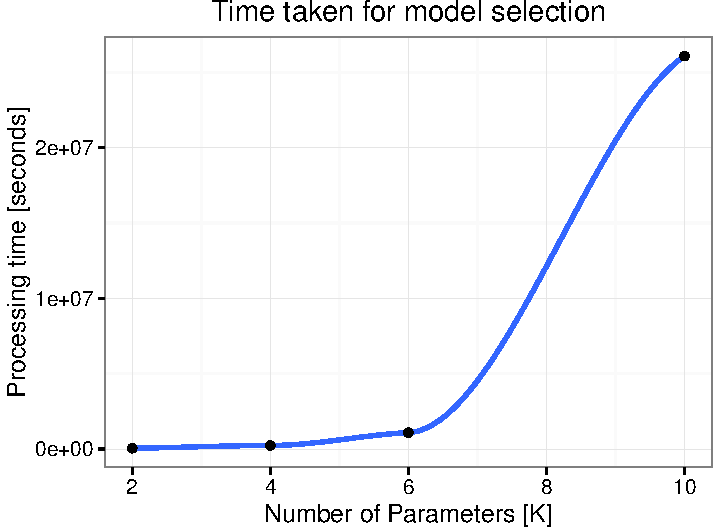
\includegraphics{diversityocc_files/figure-latex/unnamed-chunk-13-1} \end{center}

\end{CodeChunk}

From now on we will work with automatically selected models for bird
abundance and diversity using an information theoretic approach (AICc).

\begin{CodeChunk}
\begin{CodeInput}
birdmodel.selected <- diversityoccu(pres = IslandBirds, sitecov = siteCov,
obscov = Daily_Cov,spp =  5, form = ~ Day + Wind + Time ~ Elev + Wetland + Upland, dredge = TRUE)
\end{CodeInput}
\end{CodeChunk}

Below we present an example of an analysis with the full model (includes
all variables) and subsequently results from a model selection analysis,
both of them only for the second species:

\begin{CodeChunk}
\begin{CodeInput}
birdDiversity$models[[2]]
\end{CodeInput}
\begin{CodeOutput}

Call:
occuRN(formula = form, data = models[[i]])

Abundance:
             Estimate       SE      z P(>|z|)
(Intercept)   0.66046 7.41e-01  0.891  0.3731
Elev         -0.00398 1.73e-03 -2.305  0.0212
Wetland     -47.31278 1.72e+02 -0.276  0.7828
Upland       -0.42087 5.56e-01 -0.756  0.4494

Detection:
            Estimate      SE      z P(>|z|)
(Intercept) -2.36626 1.80923 -1.308  0.1909
Day          0.03480 0.01801  1.932  0.0534
Wind        -0.10959 0.19166 -0.572  0.5675
Time        -0.00114 0.00375 -0.305  0.7605

AIC: 208.1134 
\end{CodeOutput}
\begin{CodeInput}
birdmodel.selected$models[[2]]
\end{CodeInput}
\begin{CodeOutput}

Call:
occuRN(formula = ~Day + 1 ~ Elev + Wetland + 1, data = data2)

Abundance:
            Estimate      SE      z P(>|z|)
(Intercept)  0.50953 0.66082  0.771 0.44067
Elev        -0.00446 0.00164 -2.725 0.00643
Wetland     -5.05318 2.71875 -1.859 0.06308

Detection:
            Estimate     SE     z  P(>|z|)
(Intercept)  -3.1681 0.8008 -3.96 7.62e-05
Day           0.0324 0.0174  1.86 6.29e-02

AIC: 204.0382 
\end{CodeOutput}
\end{CodeChunk}

The responses of individual species to specific variables can be shown
using the function responseplot.abund.abund, bellow we show the response
of abundance in species 2 to the Burn intensity soil. Note that this
function automatically bounds the limits of the variable to the maximum
and minimum observable values in the field.

\begin{CodeChunk}
\begin{CodeInput}
responseplot.abund(birdmodel.selected, spp = 2, variable = Elev)
\end{CodeInput}


\begin{center}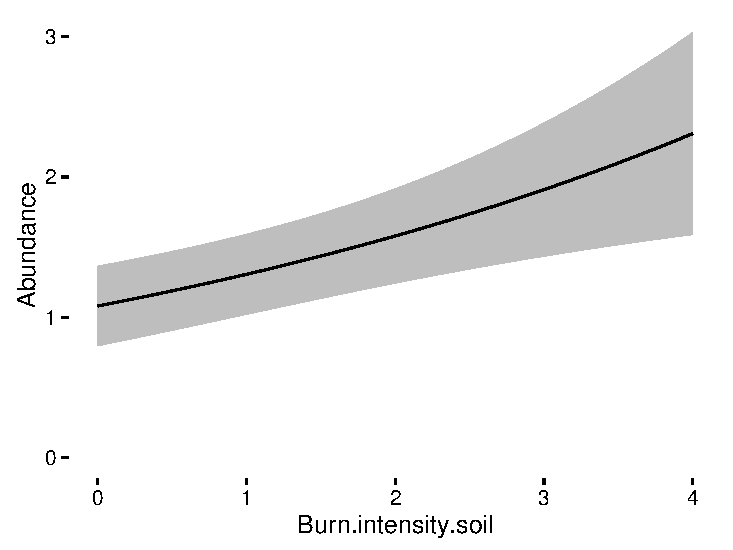
\includegraphics{diversityocc_files/figure-latex/unnamed-chunk-16-1} \end{center}

\end{CodeChunk}

\subsection{Model selection for alpha diversity
modeling}\label{model-selection-for-alpha-diversity-modeling}

The next step is to select the best model for predicting alpha diversity
using the model.diversity function. The function takes a
diversityoccupancy object, and fits all possible glm models and ranks
them by AICc. Other than the diversityoccupancy object, there are three
other parameters to select: 1) Method, which can be either ``h'' which
fits every possible model, or ``g'', which uses genetic algorithms to
select models (recommended for large candidate sets); 2) Delta, which
allows the user to identify an AICc delta threshold, which returns all
models with AICc values below the threshold; 3) Squared, which includes
only linear combinations when set to FALSE (Default), and both linear
and quadratic (second order) if set to TRUE.

\begin{CodeChunk}
\begin{CodeInput}
glm.BirdDiverse <- model.diversity(birdmodel.selected, method = "g", delta = 2, 
squared = TRUE)
\end{CodeInput}
\end{CodeChunk}

To see the top models extract the Table element of the modelselection
object

\textbackslash{}begin\{CodeChunk\} \textbackslash{}begin\{CodeOutput\}
model 1 Diversity \textasciitilde{} 1 + Elev + AgroFo + Wetland +
I(Elev\^{}2) + I(AgroFo\^{}2) + I(SecVec\^{}2) + I(Wetland\^{}2) +
I(Upland\^{}2) 2 Diversity \textasciitilde{} 1 + Elev + AgroFo + Wetland
+ I(Elev\^{}2) + I(AgroFo\^{}2) + I(Wetland\^{}2) + I(Upland\^{}2) 3
Diversity \textasciitilde{} 1 + Elev + AgroFo + Wetland + Upland +
I(Elev\^{}2) + I(AgroFo\^{}2) + I(Wetland\^{}2) + I(Upland\^{}2) 4
Diversity \textasciitilde{} 1 + Elev + SecVec + Wetland + Upland +
I(Elev\^{}2) + I(AgroFo\^{}2) + I(Wetland\^{}2) + I(Upland\^{}2) 5
Diversity \textasciitilde{} 1 + Elev + AgroFo + SecVec + Wetland +
I(Elev\^{}2) + I(AgroFo\^{}2) + I(Wetland\^{}2) + I(Upland\^{}2) aicc
weights Delta.AICc 1 -681.3992 0.2610582 0.0000000 2 -681.1351 0.2287691
0.2640605 3 -680.7723 0.1908161 0.6268668 4 -680.4609 0.1632999
0.9383094 5 -680.3701 0.1560568 1.0290469
\textbackslash{}end\{CodeOutput\} \textbackslash{}end\{CodeChunk\}

The responseplot.diver function takes a modeldiversity object and one of
the variables used to predict the alpha diversity index, and makes a
plot showing the response of the diversity index against the selected
variable. This function automatically limits the values of that variable
to the maximum and minimum values of the dataset. It also shows the
standard deviation of the estimation.

\begin{CodeChunk}
\begin{CodeInput}
responseplot.diver(glm.BirdDiverse, Elev)
\end{CodeInput}


\begin{center}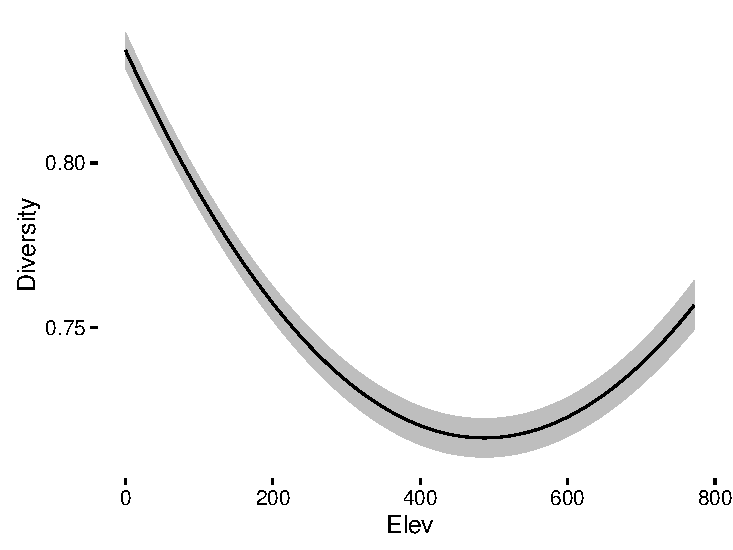
\includegraphics{diversityocc_files/figure-latex/unnamed-chunk-19-1} \end{center}

\end{CodeChunk}

Also since the returned plot is a ggplot type object, it can be easily
modified following ggplot2 grammar of graphics.

\begin{CodeChunk}
\begin{CodeInput}
library(ggplot2)
k <- responseplot.diver(glm.BirdDiverse, Elev)
k
\end{CodeInput}


\begin{center}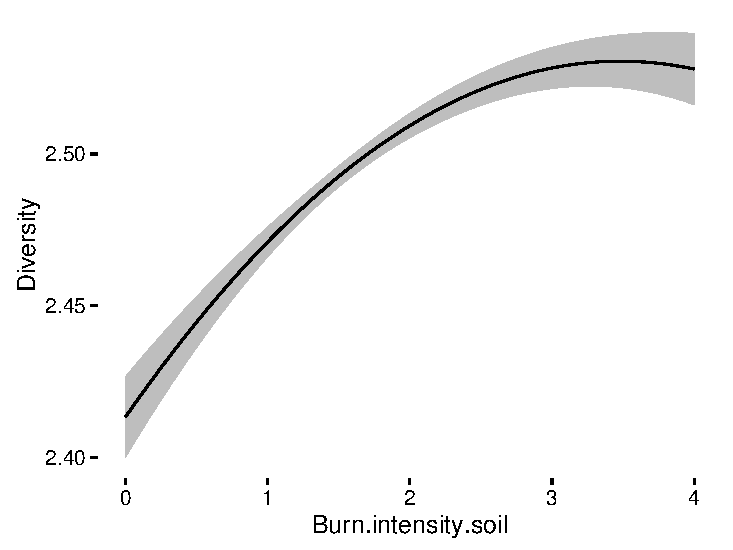
\includegraphics{diversityocc_files/figure-latex/unnamed-chunk-20-1} \end{center}

\begin{CodeInput}
k + theme_gray()
\end{CodeInput}


\begin{center}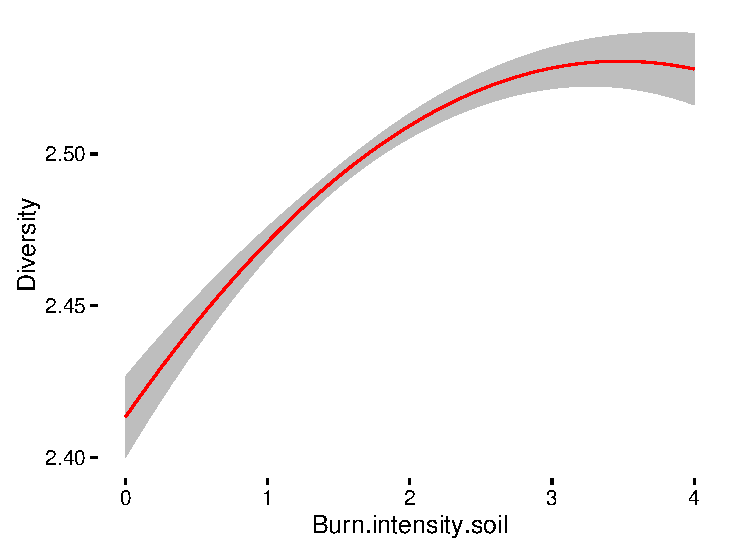
\includegraphics{diversityocc_files/figure-latex/unnamed-chunk-20-2} \end{center}

\begin{CodeInput}
k + ylim(c(0,1))
\end{CodeInput}


\begin{center}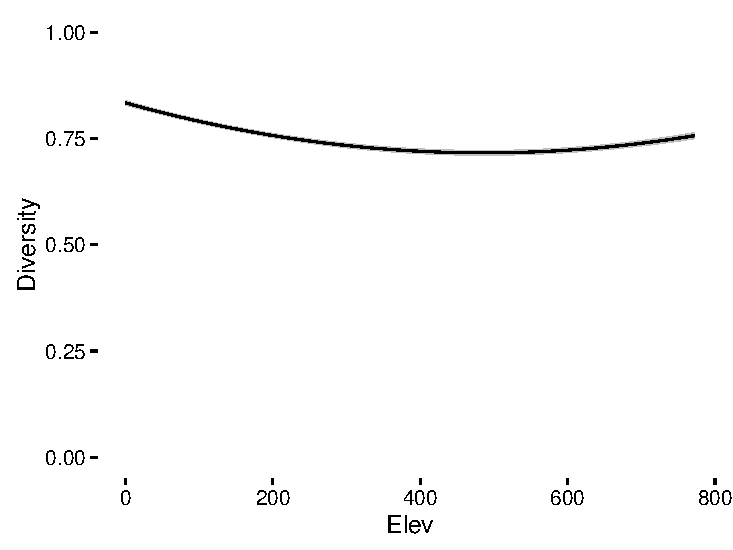
\includegraphics{diversityocc_files/figure-latex/unnamed-chunk-20-3} \end{center}

\end{CodeChunk}

\subsection{Selecting conservation areas based on alpha diversity and
abundance of species of conservation
concern}\label{selecting-conservation-areas-based-on-alpha-diversity-and-abundance-of-species-of-conservation-concern}

Of the 5 species modeled, lets say that there are at least two of
conservation concern, the second and thirds of our list. Since we
already have models relating site characteristics to species abundance
and a model relating site characteristics to alpha diversity, with the
use of a spatial raster layers (rasterstack) with the modeled variables
we can choose an area with high species diversity and/or abundance. In
order for this function to work properly the stack has to be in lon lat
projection, and Birdstack is in UTM, so we reproject the data.

\begin{CodeChunk}
\begin{CodeInput}
library(raster)
\end{CodeInput}
\begin{CodeOutput}
Loading required package: sp
\end{CodeOutput}
\begin{CodeOutput}

Attaching package: 'sp'
\end{CodeOutput}
\begin{CodeOutput}
The following object is masked from 'package:unmarked':

    coordinates
\end{CodeOutput}
\begin{CodeOutput}

Attaching package: 'raster'
\end{CodeOutput}
\begin{CodeOutput}
The following objects are masked from 'package:unmarked':

    getData, projection
\end{CodeOutput}
\begin{CodeInput}
data(Birdstack)
plot(Birdstack)
\end{CodeInput}


\begin{center}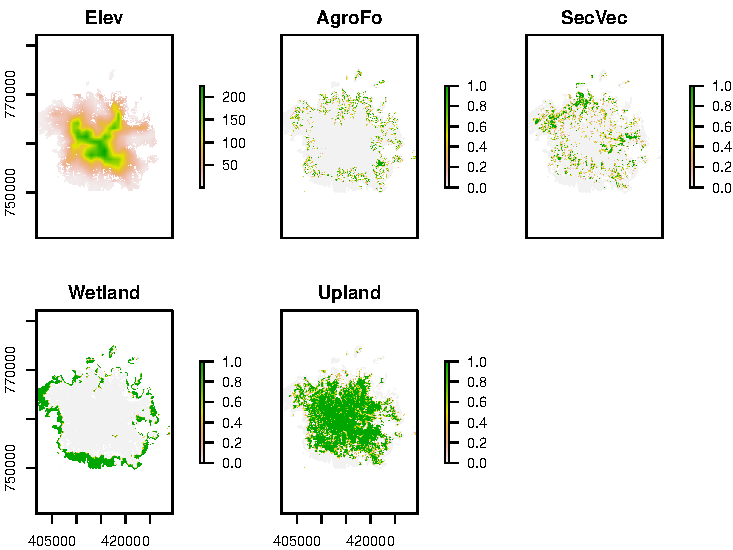
\includegraphics{diversityocc_files/figure-latex/unnamed-chunk-21-1} \end{center}

\begin{CodeInput}
newproj <- '+proj=longlat +datum=WGS84 +ellps=WGS84 +towgs84=0,0,0'
library(rgdal)
\end{CodeInput}
\begin{CodeOutput}
rgdal: version: 1.1-10, (SVN revision 622)
 Geospatial Data Abstraction Library extensions to R successfully loaded
 Loaded GDAL runtime: GDAL 2.0.1, released 2015/09/15
 Path to GDAL shared files: C:/Users/corcoranbarriosd/Documents/R/win-library/3.2/rgdal/gdal
 GDAL does not use iconv for recoding strings.
 Loaded PROJ.4 runtime: Rel. 4.9.1, 04 March 2015, [PJ_VERSION: 491]
 Path to PROJ.4 shared files: C:/Users/corcoranbarriosd/Documents/R/win-library/3.2/rgdal/proj
 Linking to sp version: 1.2-3 
\end{CodeOutput}
\begin{CodeInput}
Birdstack <- stack(projectRaster(Birdstack, crs=newproj))
\end{CodeInput}
\end{CodeChunk}

In order to find areas of high conservation value, we use the
predict.diversity function. We need both a diversityoccupancy and a
modeldiversity class object, used in the model, and diverse parameters
respectfully, a spatial representation of site covariates as raster
files (rasterstack), with the variables in the new.data parameter, a
boolean vector in the species parameter indicating which species shall
be considered (T or F), and the quantile.nth parameter, which indicates
a quantile threshold that is used for abundance and/or richness to
indicate conservation value (areas above the threshold will be
returned).

\begin{CodeChunk}
\begin{CodeInput}
Selected.area <- diversity.predict(model = birdmodel.selected, diverse = glm.BirdDiverse, new.data = Birdstack, quantile.nth = 0.65, species =
c(F,T,T,F,F))
\end{CodeInput}


\begin{center}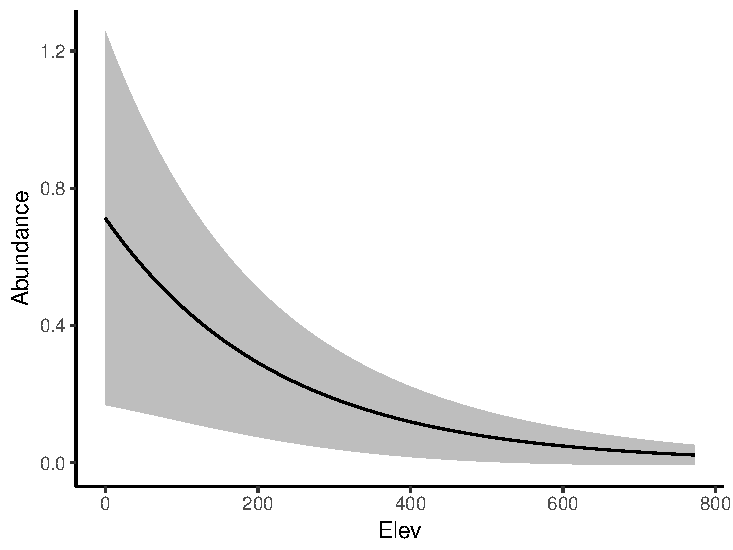
\includegraphics{diversityocc_files/figure-latex/unnamed-chunk-22-1} \end{center}

\end{CodeChunk}

From the object Selected.area we can extract and plot not only the area
that was selected with the atributes, but also the layers that shoe the
predicted diversity for the island and also the predicted abundance for
each of the species that were used for the analysis.

\section{Discussion}\label{discussion}

\renewcommand\refname{References}
\bibliography{Derek}


\end{document}

